%% ----------------------------------------------------------------
%% AppendixA.tex Circuit Diagrams
%% ---------------------------------------------------------------- 
\chapter{PCB Design} \label{Appendix:PCB}
\section{PCB Top Side}
\begin{figure}[ht!]
\centering
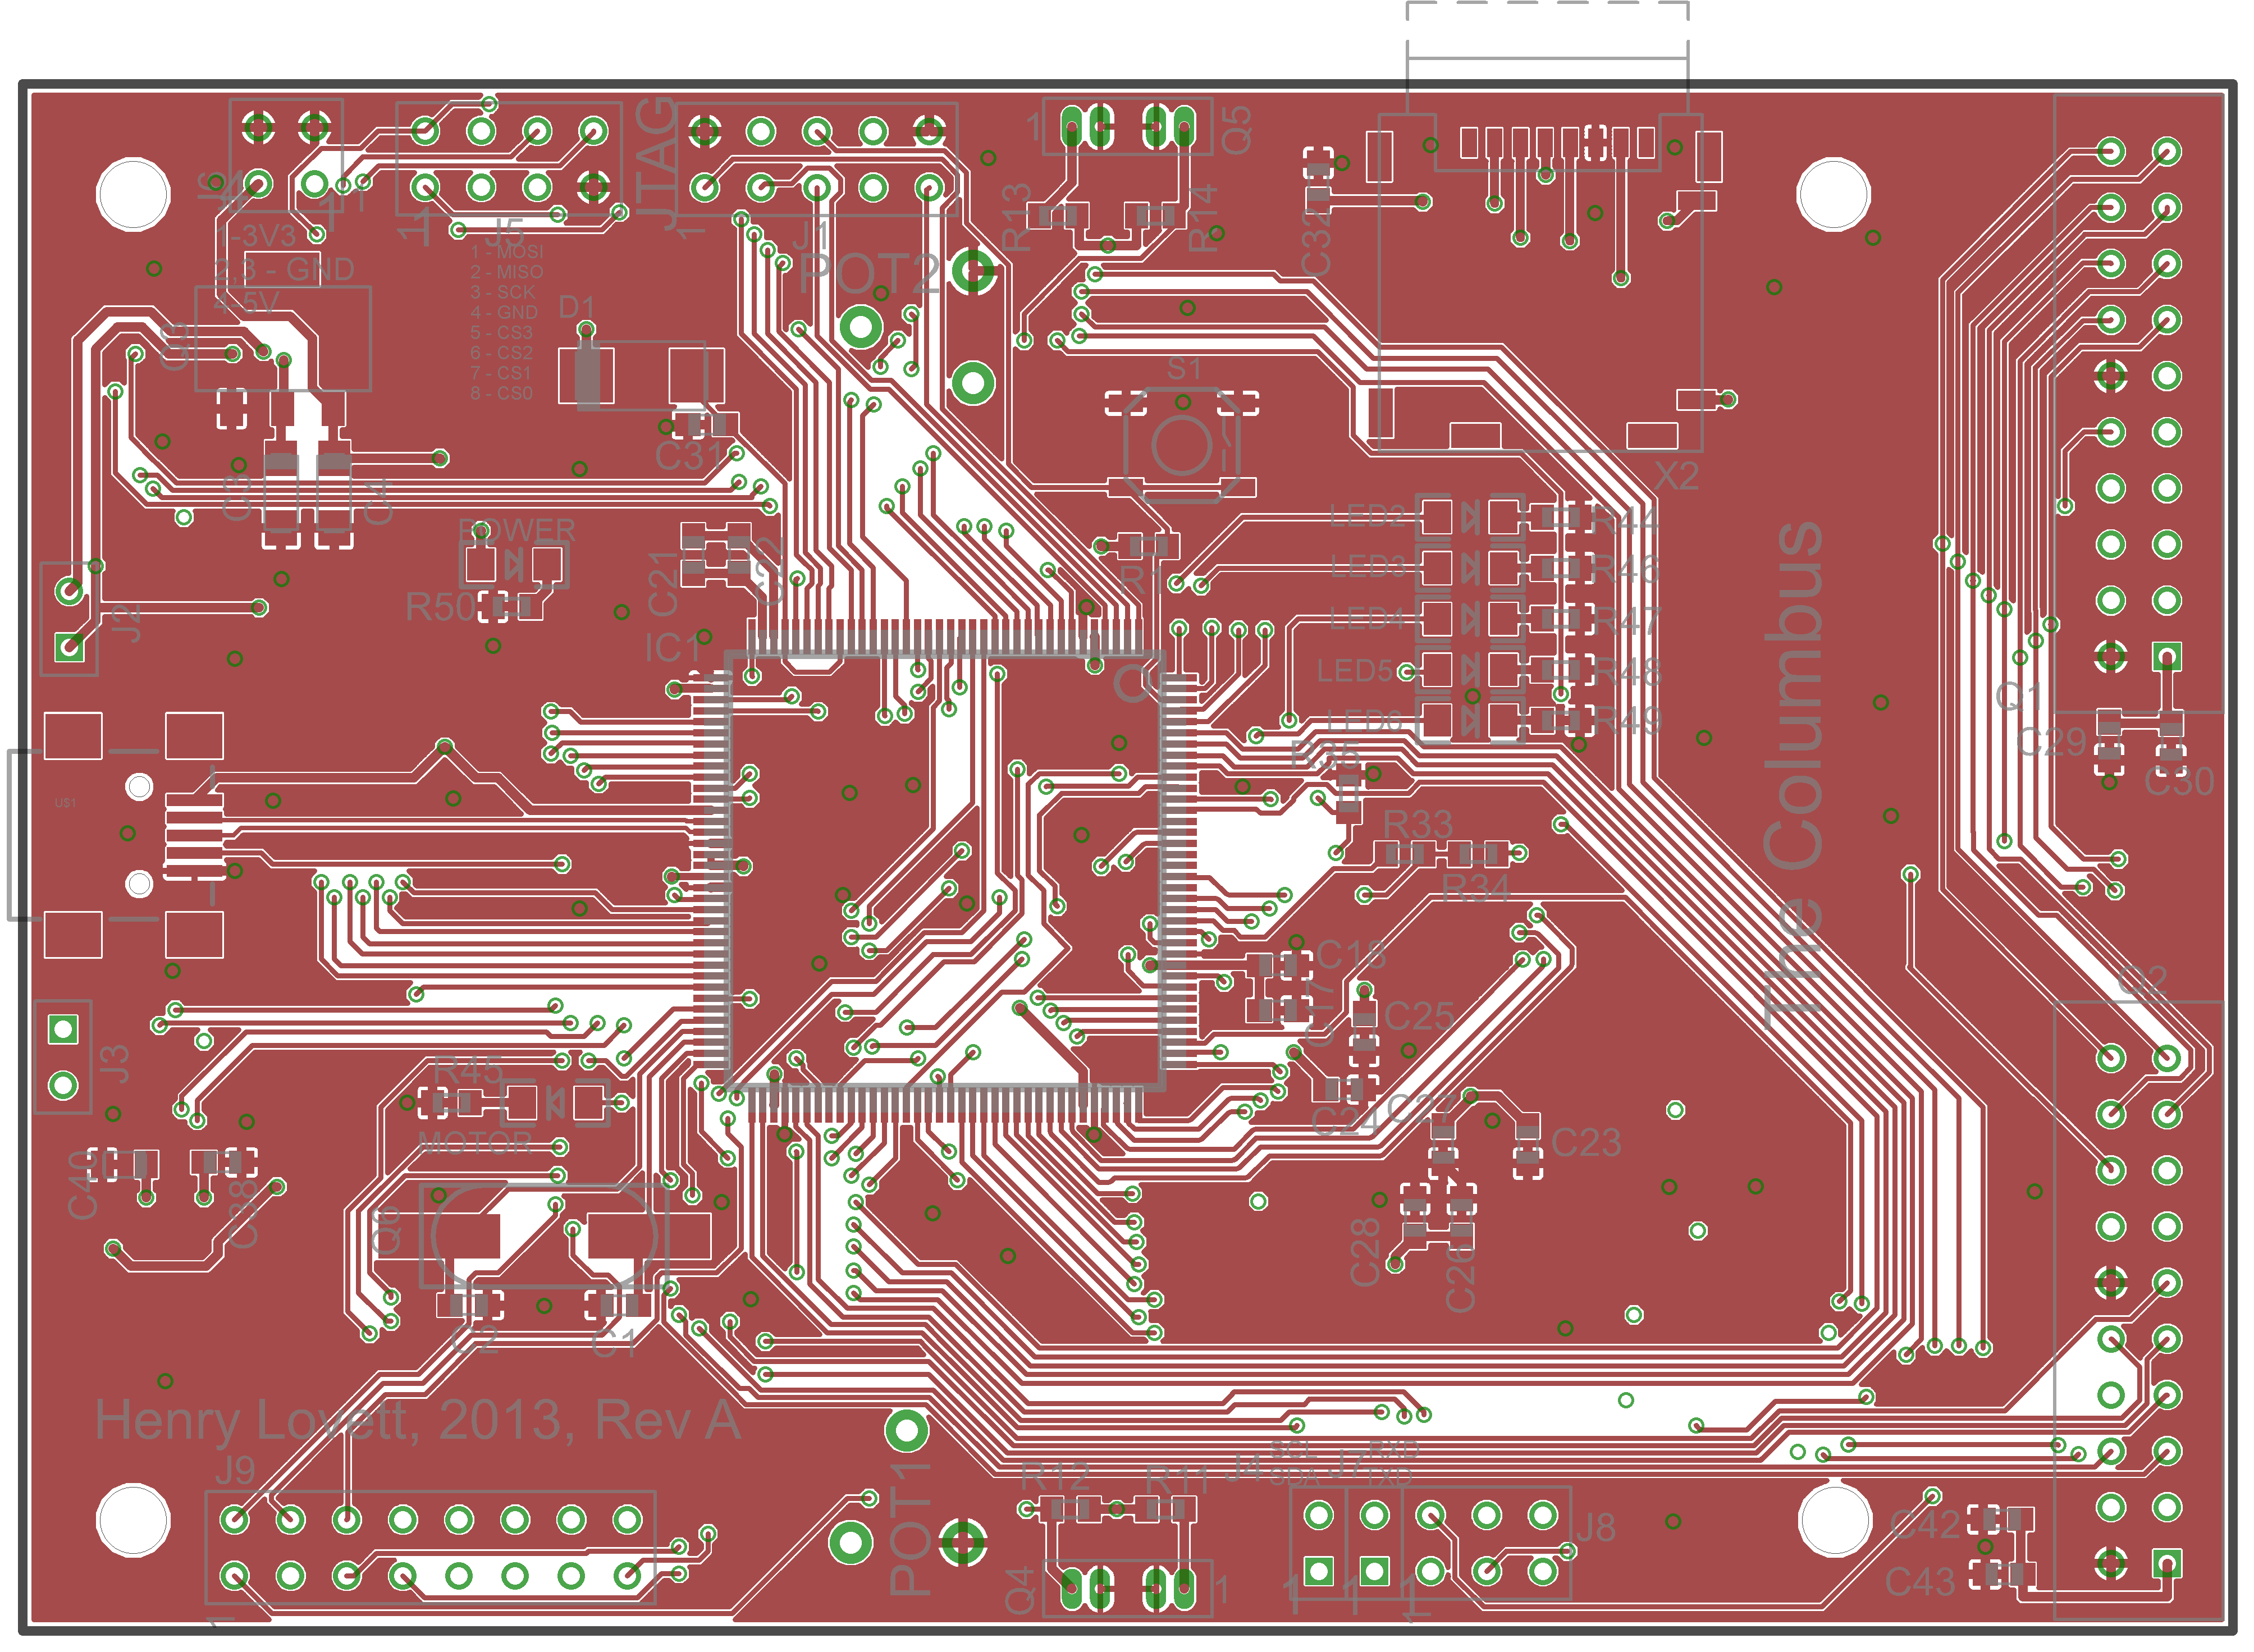
\includegraphics[angle=90,width=\textwidth,height=\textheight-5cm,keepaspectratio]{Figures/ColumbusPCBTop_GP.png} 
\caption{The top side of the CAD design of the PCB}
\label{fig:PCB:Eagle:Top}
\end{figure}
\clearpage
\section{PCB Layer 2}
\begin{figure}[ht!]
\centering
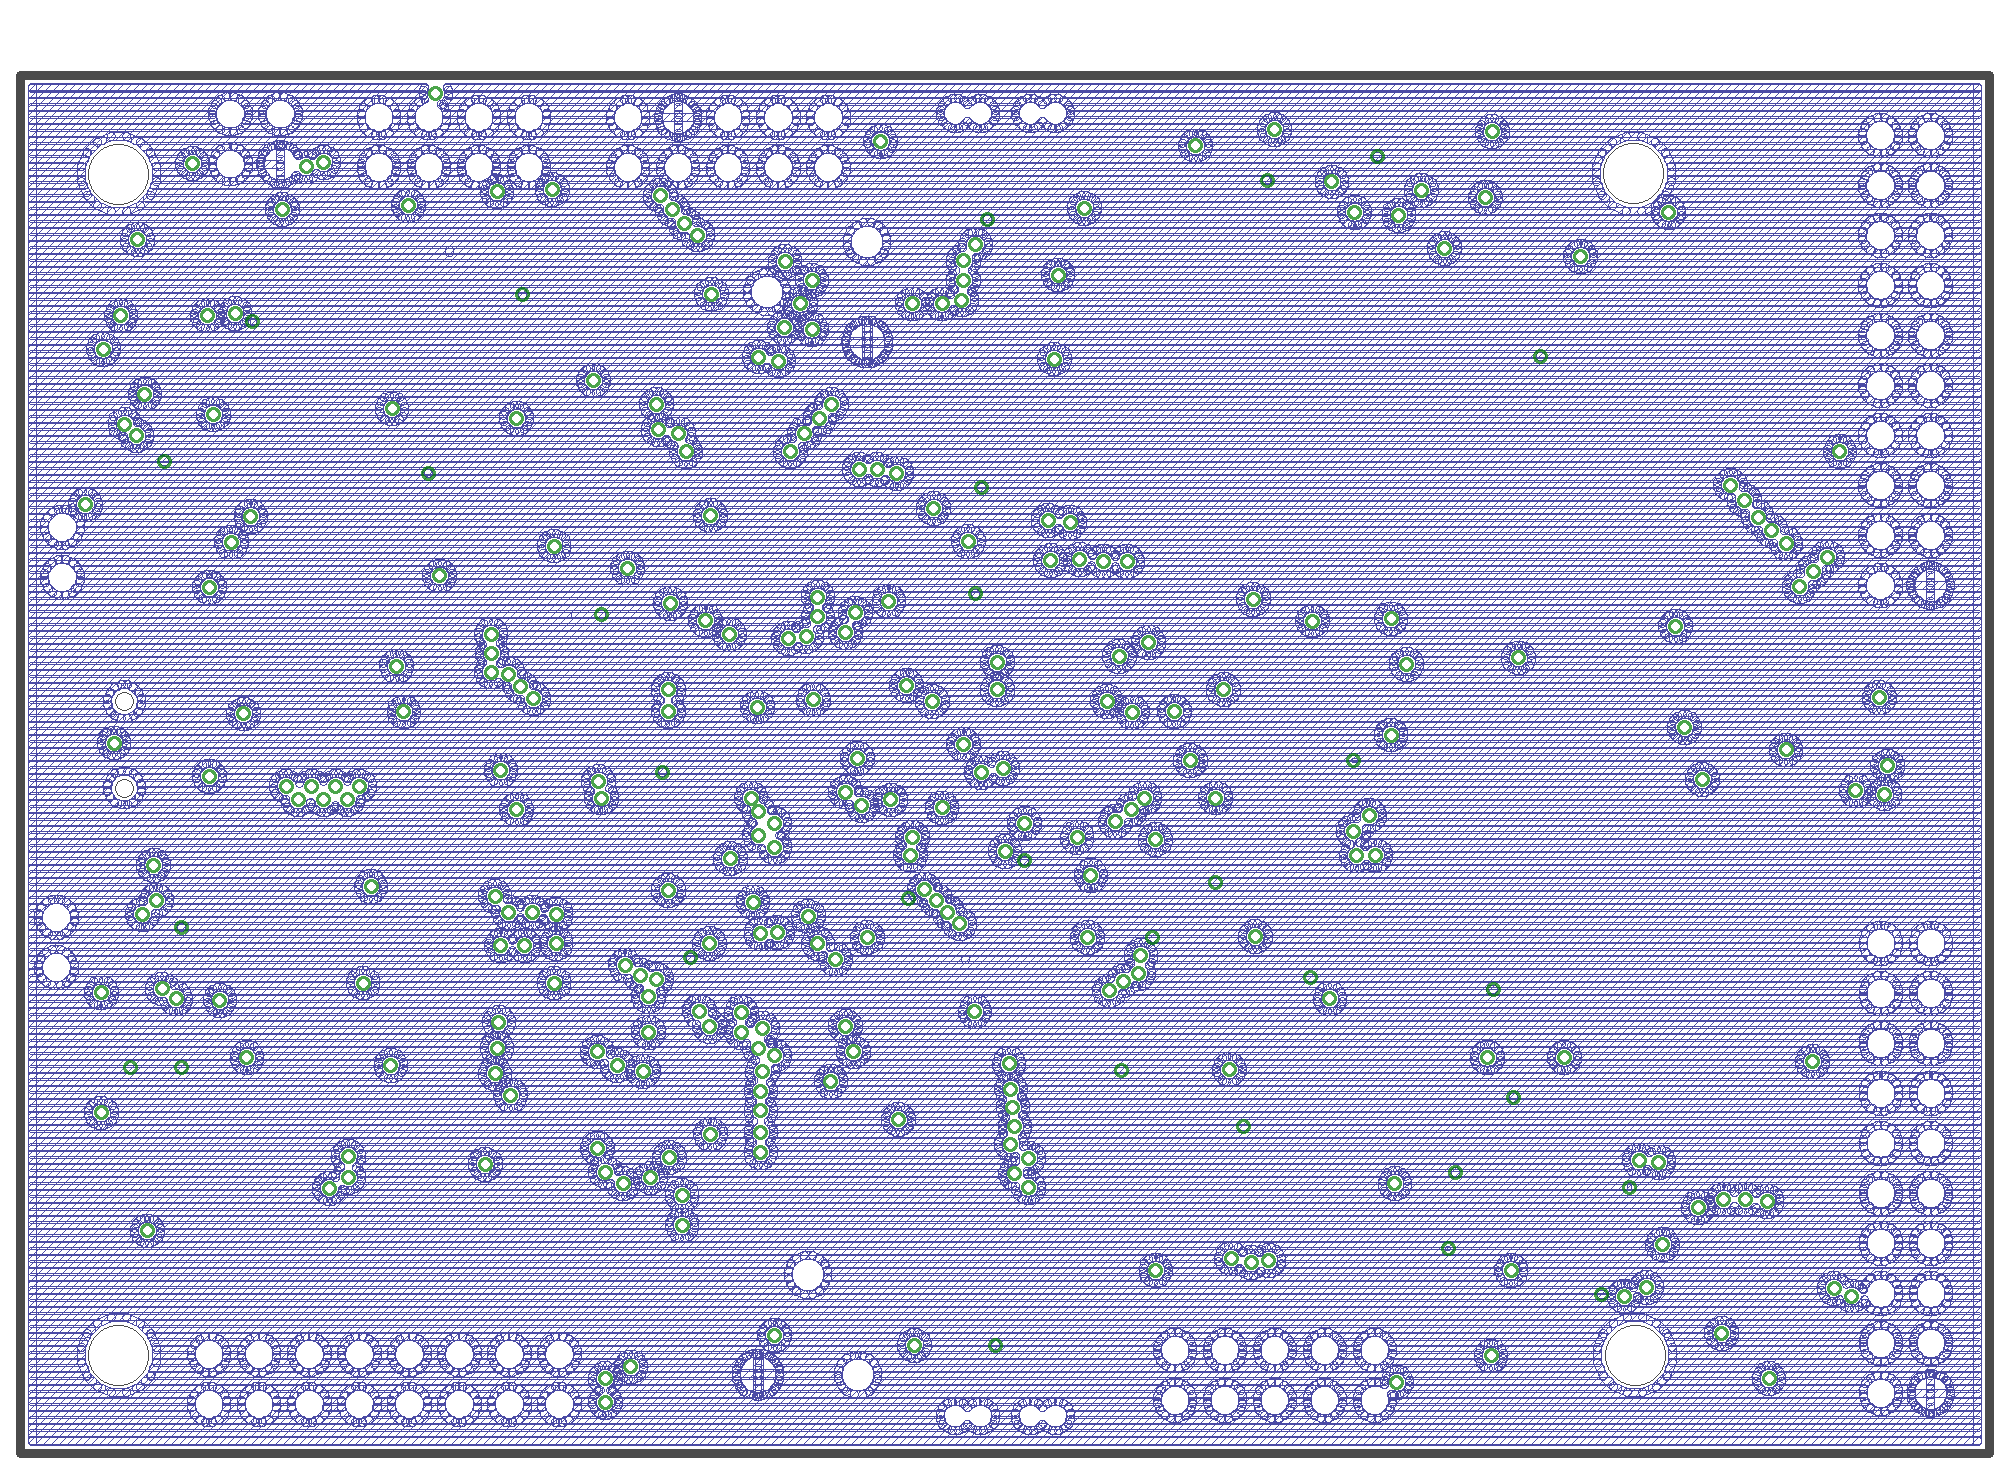
\includegraphics[angle=90,width=\textwidth,height=\textheight-5cm,keepaspectratio]{Figures/layer2.png} 
\caption{Layer 2 of the CAD design of the PCB}
\label{fig:PCB:Eagle:Bottom}
\end{figure}
\clearpage
\section{PCB Layer 3}
\begin{figure}[ht!]
\centering
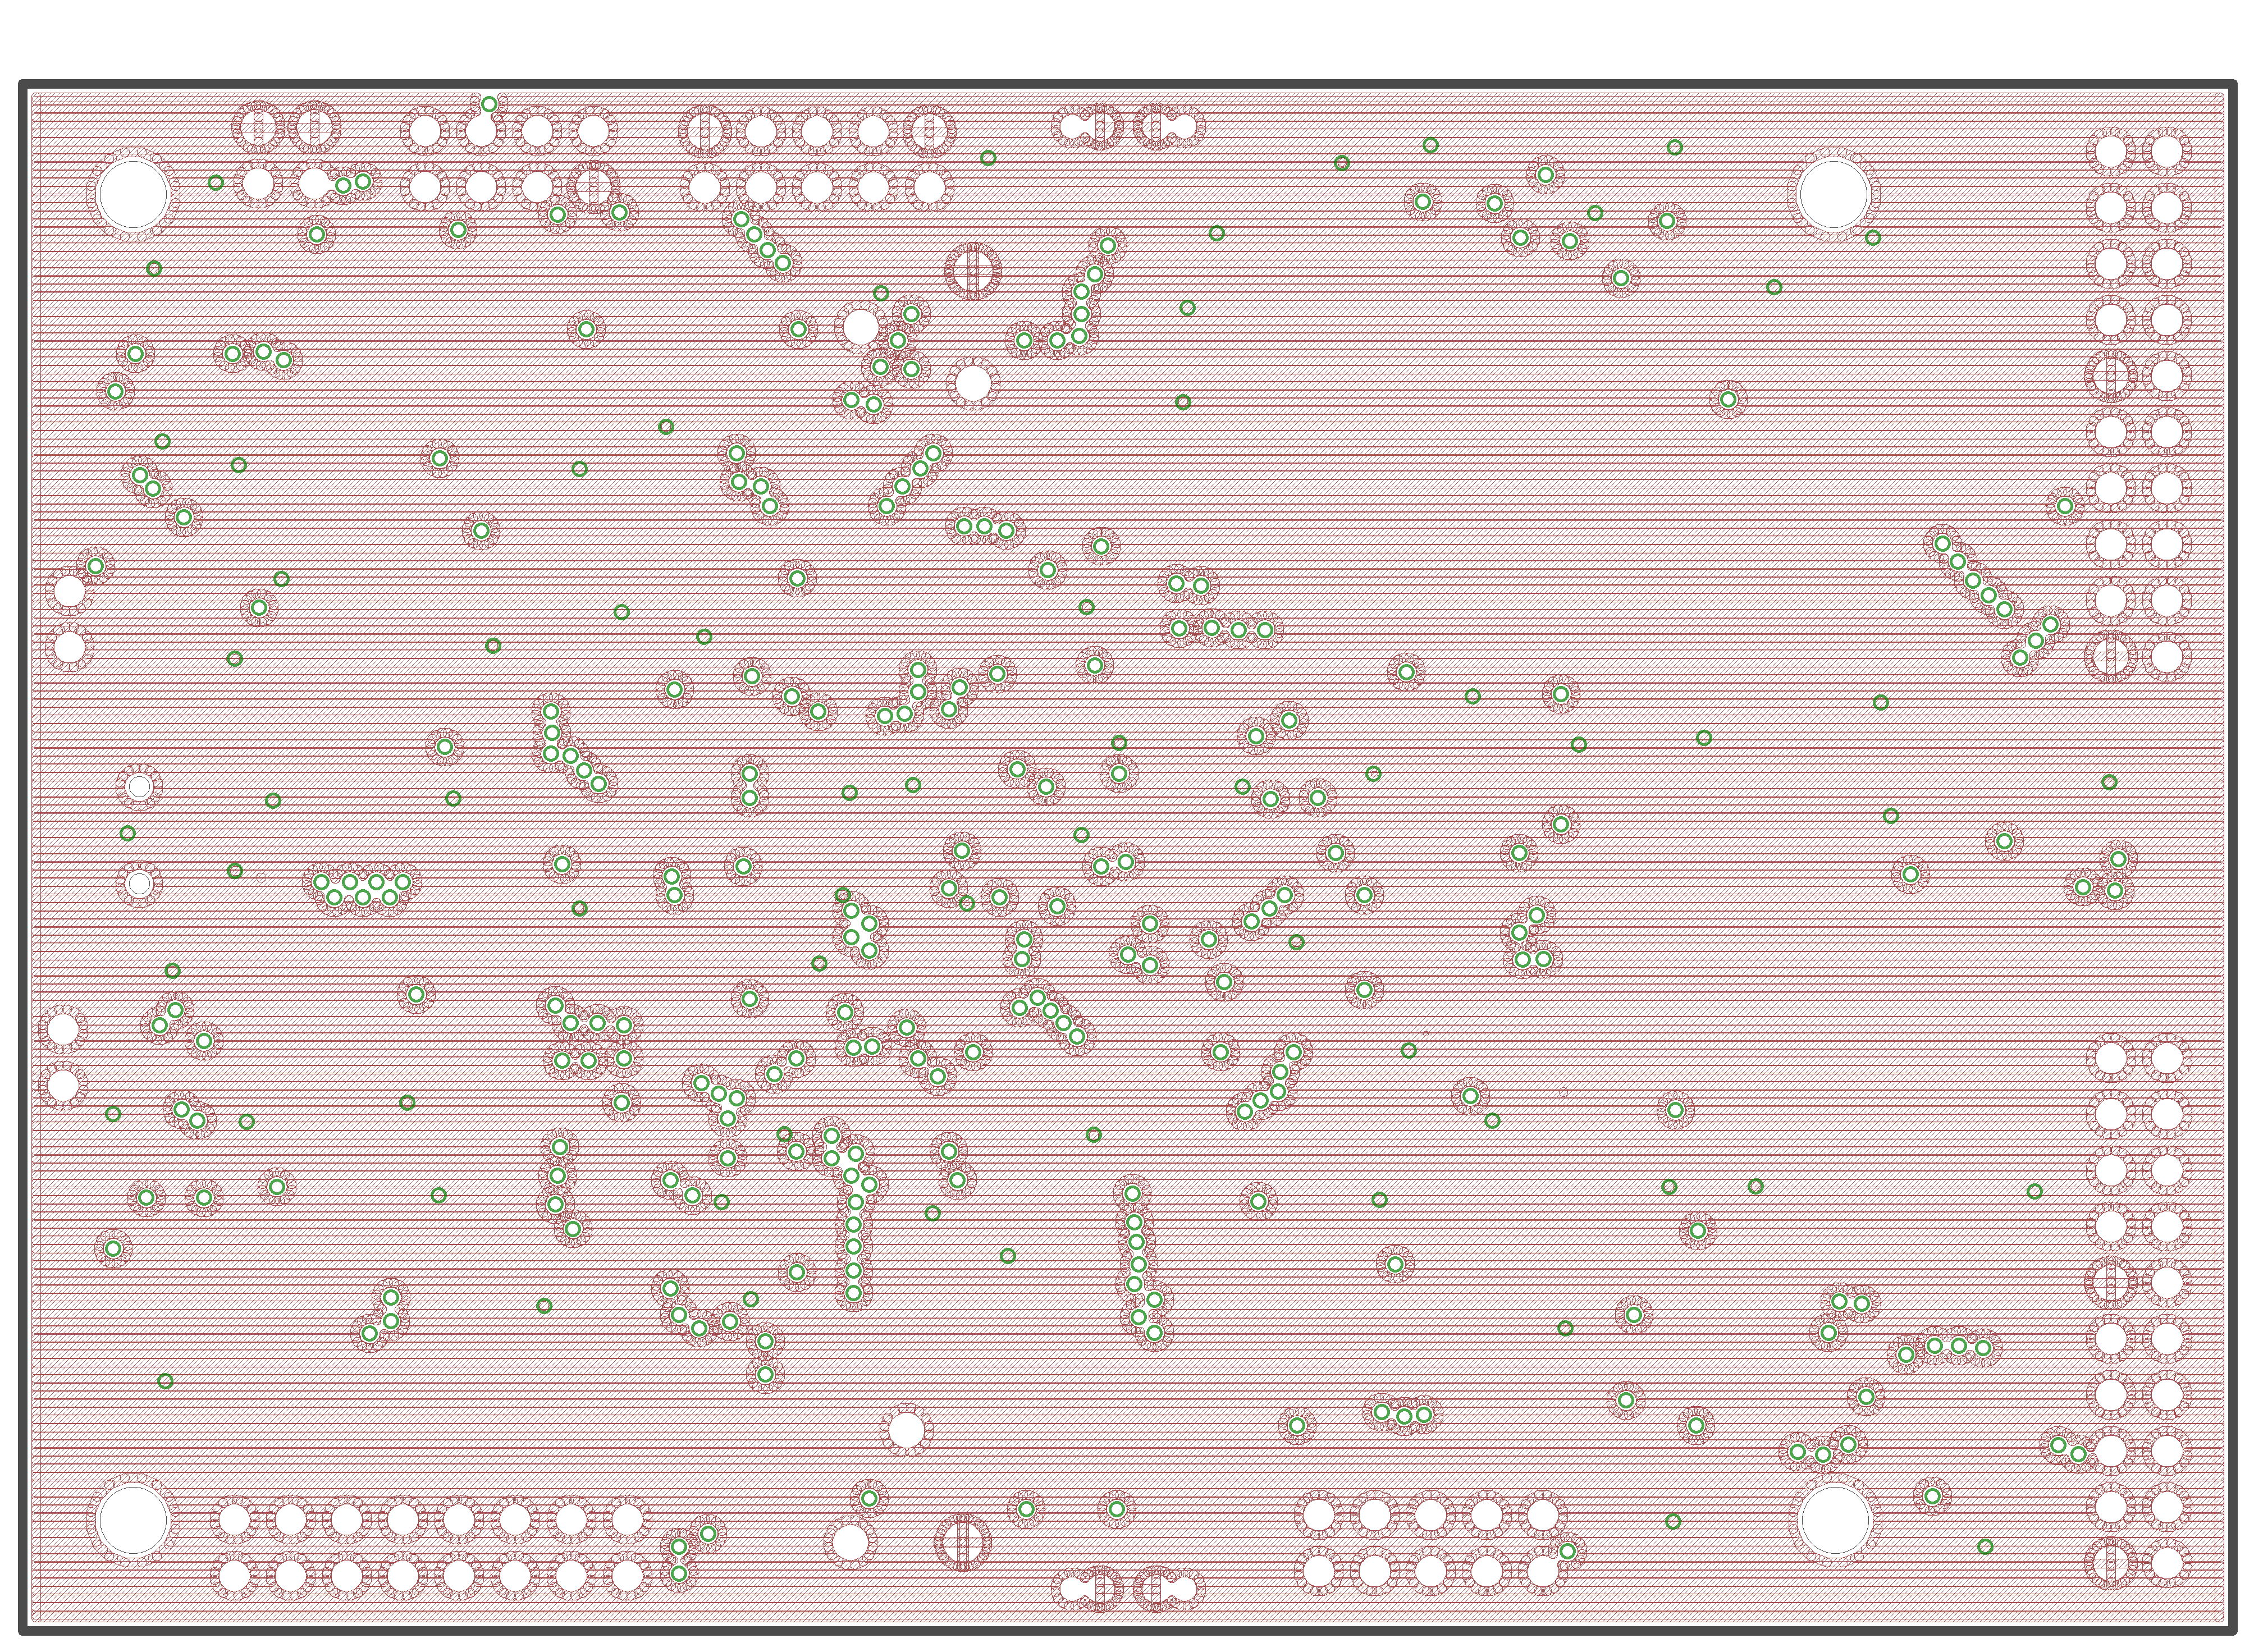
\includegraphics[angle=90,width=\textwidth,height=\textheight-5cm,keepaspectratio]{Figures/layer3.png} 
\caption{Layer 3 of the CAD design of the PCB}
\label{fig:PCB:Eagle:Bottom}
\end{figure}
\clearpage
\section{PCB Bottom Side}
\begin{figure}[ht!]
\centering
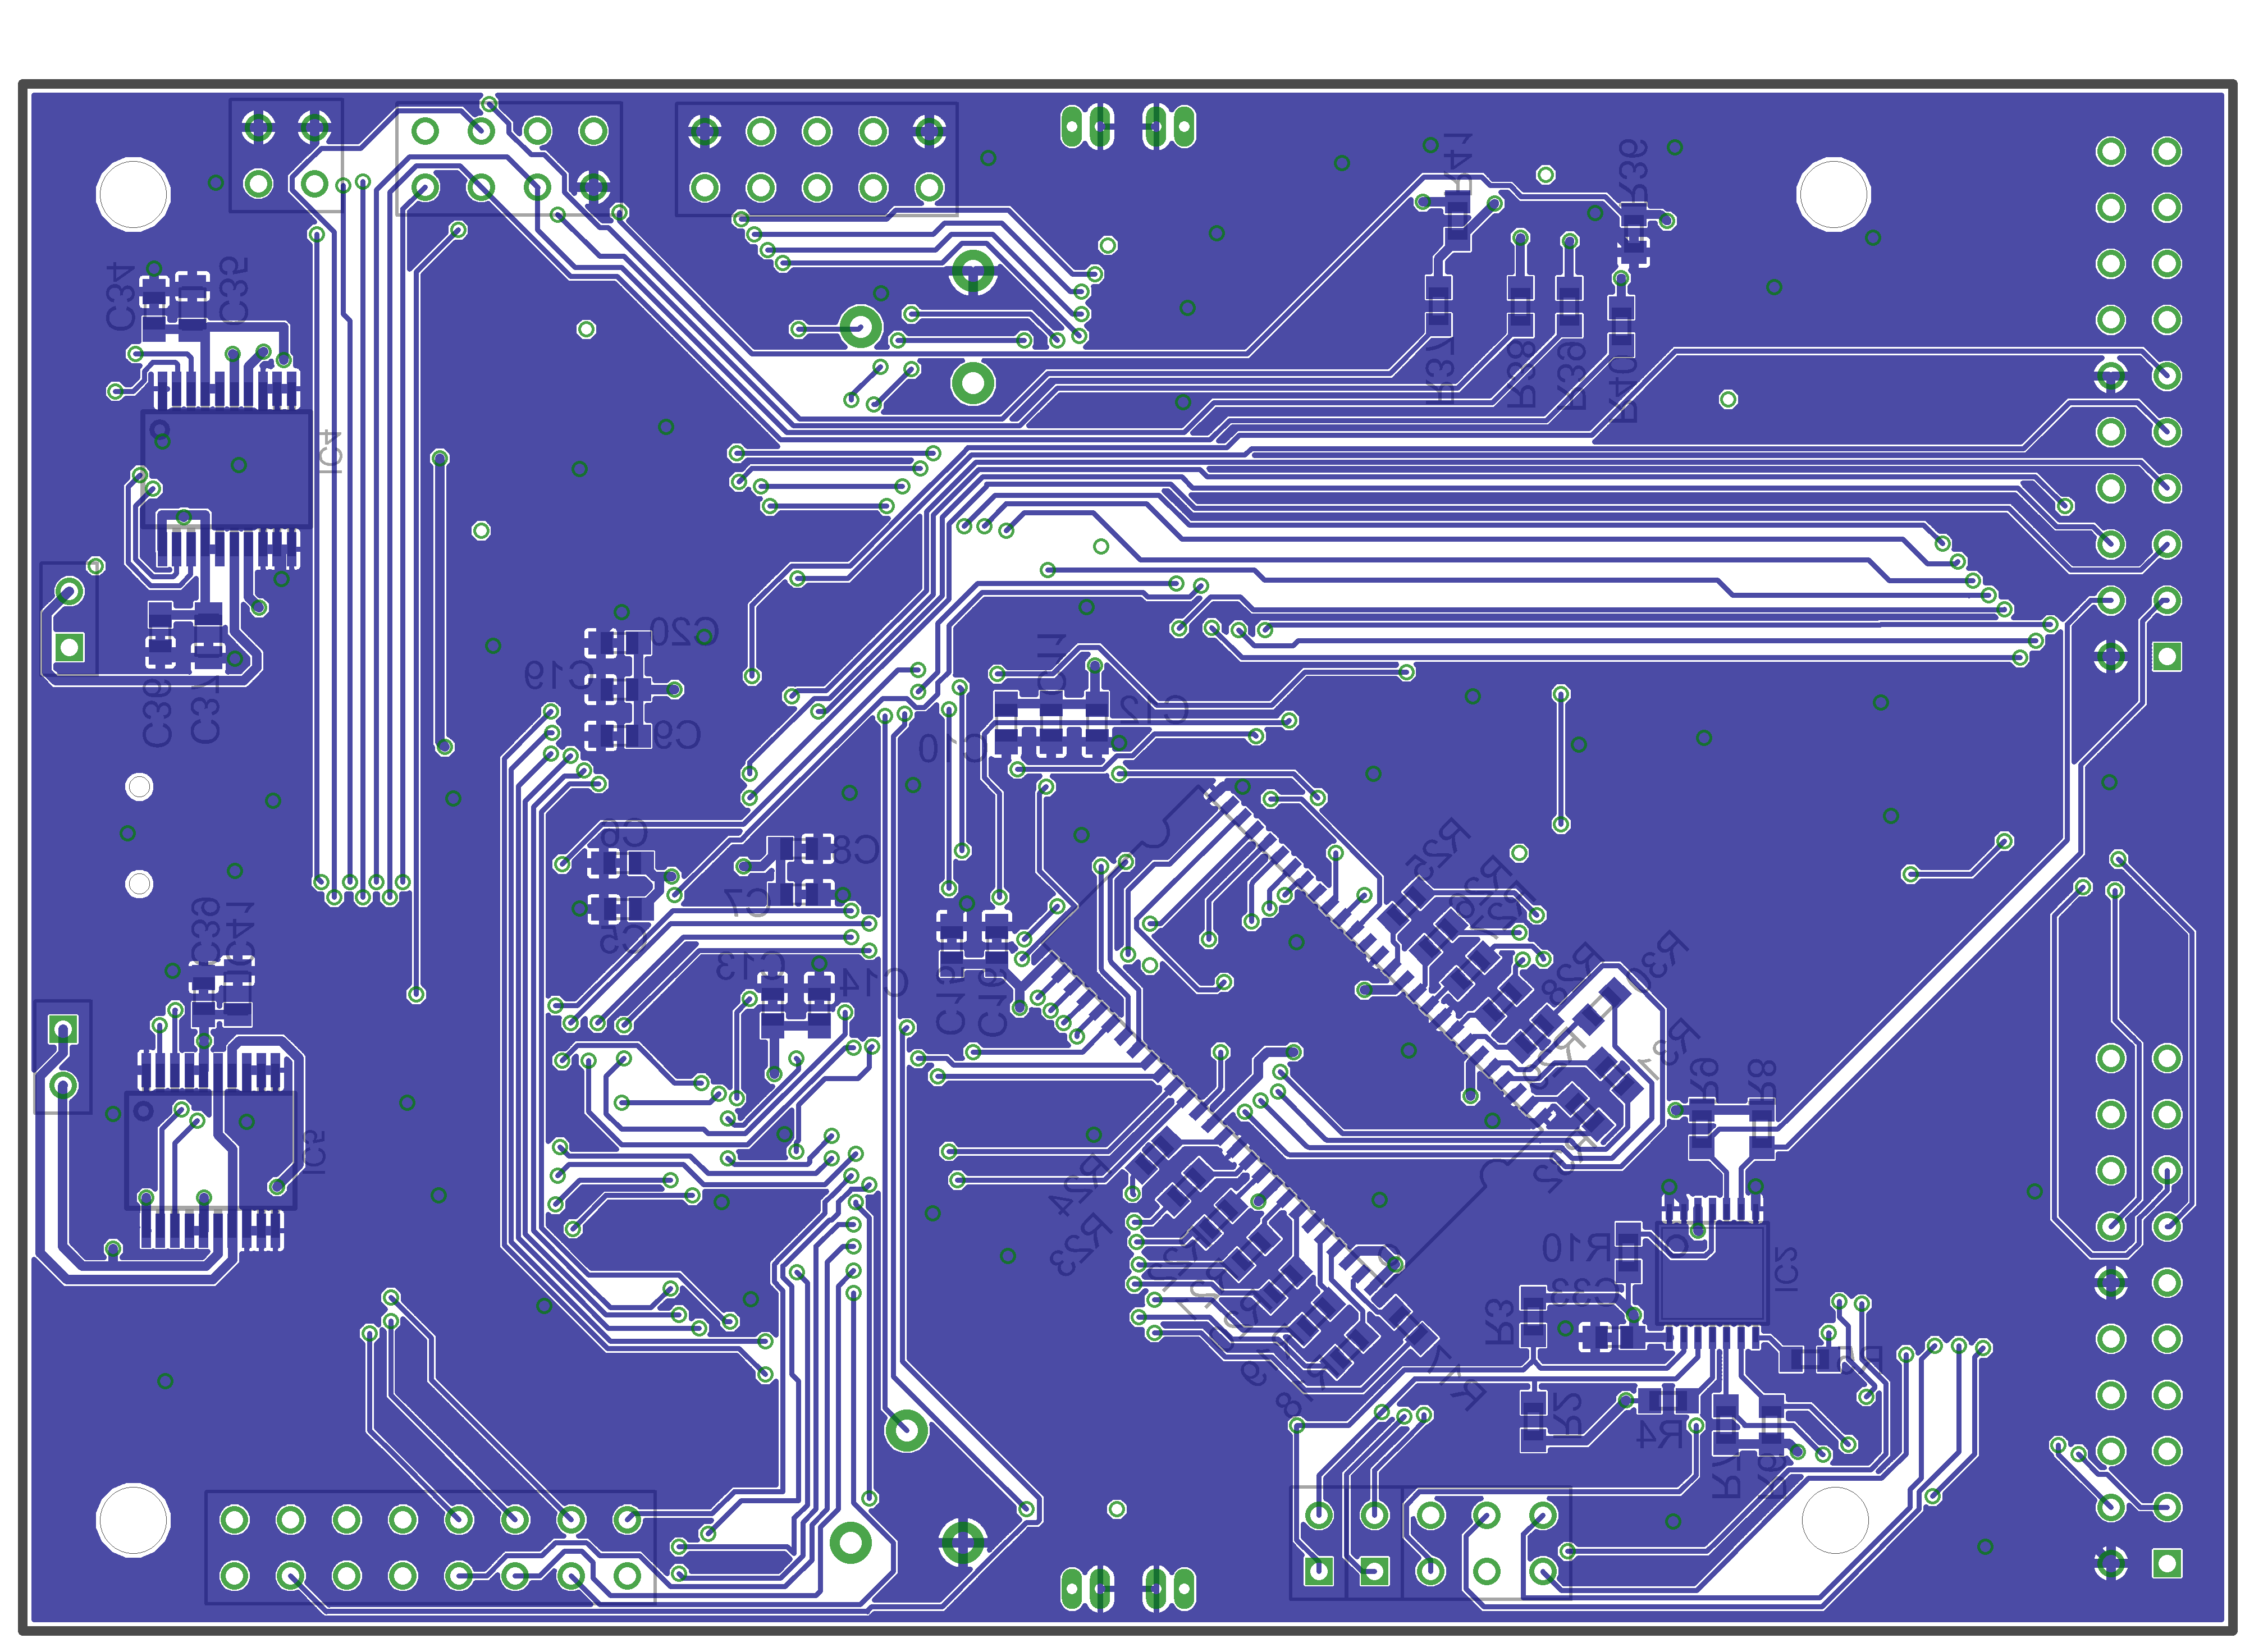
\includegraphics[angle=90,width=\textwidth,height=\textheight-5cm,keepaspectratio]{Figures/ColumbusPCBBottom_GP.png} 
\caption{The bottom side of the CAD design of the PCB}
\label{fig:PCB:Eagle:Bottom}
\end{figure}
\clearpage